\documentclass[journal,12pt,twocolumn]{IEEEtran}

\usepackage{setspace}
\usepackage{gensymb}
\singlespacing
\usepackage[cmex10]{amsmath}
\usepackage{amssymb}
\usepackage{xurl}
\usepackage{tabularx}
\usepackage{amsthm}
\usepackage{comment}
\usepackage{mathrsfs}
\usepackage{txfonts}
\usepackage{stfloats}
\usepackage{bm}
\usepackage{cite}
\usepackage{cases}
\usepackage{subfig}
\usepackage{arydshln}
\usepackage{longtable}
\usepackage{multirow}

\usepackage{enumitem}
\usepackage{mathtools}
\usepackage{steinmetz}
\usepackage{tikz}
\usepackage{circuitikz}
\usepackage{verbatim}
\usepackage{tfrupee}
\usepackage[breaklinks=true]{hyperref}
\usepackage{graphicx}
\usepackage{tkz-euclide}
\usetikzlibrary{automata, positioning}
\usetikzlibrary{calc,math}
\usepackage{listings}
    \usepackage{color}                                            %%
    \usepackage{array}                                            %%
    \usepackage{longtable}                                        %%
    \usepackage{calc}                                             %%
    \usepackage{multirow}                                         %%
    \usepackage{hhline}                                           %%
    \usepackage{ifthen}                                           %%
    \usepackage{lscape}     
\usepackage{multicol}
\usepackage{chngcntr}
\usepackage{blkarray}

\DeclareMathOperator*{\Res}{Res}

\renewcommand\thesection{\arabic{section}}
\renewcommand\thesubsection{\thesection.\arabic{subsection}}
\renewcommand\thesubsubsection{\thesubsection.\arabic{subsubsection}}

\renewcommand\thesectiondis{\arabic{section}}
\renewcommand\thesubsectiondis{\thesectiondis.\arabic{subsection}}
\renewcommand\thesubsubsectiondis{\thesubsectiondis.\arabic{subsubsection}}


\hyphenation{op-tical net-works semi-conduc-tor}
\def\inputGnumericTable{}                                 %%

\lstset{
%language=C,
frame=single, 
breaklines=true,
columns=fullflexible
}
\begin{document}


\newtheorem{theorem}{Theorem}[section]
\newtheorem{problem}{Problem}
\newtheorem{proposition}{Proposition}[section]
\newtheorem{lemma}{Lemma}[section]
\newtheorem{corollary}[theorem]{Corollary}
\newtheorem{example}{Example}[section]
\newtheorem{definition}[problem]{Definition}

\newcommand{\BEQA}{\begin{eqnarray}}
\newcommand{\EEQA}{\end{eqnarray}}
\newcommand{\define}{\stackrel{\triangle}{=}}
\bibliographystyle{IEEEtran}
\raggedbottom
\setlength{\parindent}{0pt}
\providecommand{\mbf}{\mathbf}
\providecommand{\pr}[1]{\ensuremath{\Pr\left(#1\right)}}
\providecommand{\qfunc}[1]{\ensuremath{Q\left(#1\right)}}
\providecommand{\sbrak}[1]{\ensuremath{{}\left[#1\right]}}
\providecommand{\lsbrak}[1]{\ensuremath{{}\left[#1\right.}}
\providecommand{\rsbrak}[1]{\ensuremath{{}\left.#1\right]}}
\providecommand{\brak}[1]{\ensuremath{\left(#1\right)}}
\providecommand{\lbrak}[1]{\ensuremath{\left(#1\right.}}
\providecommand{\rbrak}[1]{\ensuremath{\left.#1\right)}}
\providecommand{\cbrak}[1]{\ensuremath{\left\{#1\right\}}}
\providecommand{\lcbrak}[1]{\ensuremath{\left\{#1\right.}}
\providecommand{\rcbrak}[1]{\ensuremath{\left.#1\right\}}}
\theoremstyle{remark}
\newtheorem{rem}{Remark}
\newcommand{\sgn}{\mathop{\mathrm{sgn}}}
\providecommand{\abs}[1]{\vert#1\vert}
\providecommand{\res}[1]{\Res\displaylimits_{#1}} 
\providecommand{\norm}[1]{\lVert#1\rVert}
%\providecommand{\norm}[1]{\lVert#1\rVert}
\providecommand{\mtx}[1]{\mathbf{#1}}
\providecommand{\mean}[1]{E[ #1 ]}
\providecommand{\fourier}{\overset{\mathcal{F}}{ \rightleftharpoons}}
%\providecommand{\hilbert}{\overset{\mathcal{H}}{ \rightleftharpoons}}
\providecommand{\system}{\overset{\mathcal{H}}{ \longleftrightarrow}}
	%\newcommand{\solution}[2]{\textbf{Solution:}{#1}}
\newcommand{\solution}{\noindent \textbf{Solution: }}
\newcommand{\cosec}{\,\text{cosec}\,}
\providecommand{\dec}[2]{\ensuremath{\overset{#1}{\underset{#2}{\gtrless}}}}
\newcommand{\myvec}[1]{\ensuremath{\begin{pmatrix}#1\end{pmatrix}}}
\newcommand{\mydet}[1]{\ensuremath{\begin{vmatrix}#1\end{vmatrix}}}
\newcommand*{\permcomb}[4][0mu]{{{}^{#3}\mkern#1#2_{#4}}}
\newcommand*{\perm}[1][-3mu]{\permcomb[#1]{P}}
\newcommand*{\comb}[1][-1mu]{\permcomb[#1]{C}}
\numberwithin{equation}{subsection}
\makeatletter
\@addtoreset{figure}{problem}
\makeatother
\let\StandardTheFigure\thefigure
\let\vec\mathbf
\renewcommand{\thefigure}{\theproblem}
\def\putbox#1#2#3{\makebox[0in][l]{\makebox[#1][l]{}\raisebox{\baselineskip}[0in][0in]{\raisebox{#2}[0in][0in]{#3}}}}
     \def\rightbox#1{\makebox[0in][r]{#1}}
     \def\centbox#1{\makebox[0in]{#1}}
     \def\topbox#1{\raisebox{-\baselineskip}[0in][0in]{#1}}
     \def\midbox#1{\raisebox{-0.5\baselineskip}[0in][0in]{#1}}
\vspace{3cm}
\title{Assignment 2}
\author{Tanay Yadav - AI20BTECH11026}
\maketitle
\newpage
\bigskip
\renewcommand{\thefigure}{\theenumi}
\renewcommand{\thetable}{\theenumi}
Download the python codes from: 
%
\begin{lstlisting}
https://github.com/tanayyadav28/EE3900-Assignments/blob/main/Assignment_3/code/Assignment_3.py
\end{lstlisting}
Download the latex-tikz codes from: 
%
\begin{lstlisting}
https://github.com/tanayyadav28/EE3900-Assignments/blob/main/Assignment_3/Assignment_3.tex
\end{lstlisting}
\section{Problem}
[Construction S2; Q8]
Can you construct a quadrilateral MIST where $MI = 3.5$, $IS = 6.5$, $\angle M = 100^{\circ}$, $\angle I = 105^{\circ}$, and $\angle S = 120^{\circ}$.
\section{Solution}
Given,
\begin{align}
    \norm{\vec{MI}} &= 3.5\\
    \norm{\vec{IS}} &= 6.5\\
    \angle{TMI} &= 100^{\circ}\\
    \angle{MIS} &= 105^{\circ}\\
    \angle{IST} &= 120^{\circ}\\
\end{align}
If quadrilateral MIST is possible,
\begin{align}
    \therefore \angle{STM} &= 360 - 100 - 105 - 120\\
    \angle{STM} &= 35^{\circ}\\
    \text{Let, } \norm{\vec{ST}} &= x\\
    \norm{\vec{TM}} &= y
\end{align}\\
Considering $\vec{O} = \myvec{0\\0}$ to be the midpoint of $\vec{IS}$.
\begin{align}
    \therefore\norm{\vec{IO}} &= 3.25\\
    \norm{\vec{OS}} &= 3.25\\
\end{align}
The vectors are along the x-axis. Hence the coordinates are:
\begin{align}
    \therefore \vec{I} &= \myvec{-3.25\\0}\\
    \vec{S} &= \myvec{3.25\\0}
\end{align}
\begin{align}
    \because \angle MIS &= 105^{\circ}\\
    \therefore \vec{M} &= \myvec{-3.25 + \norm{{\vec{MI}}}\cos({\angle{MIS}})\\0 + \norm{\vec{MI}}\sin({\angle{MIS}})}\\
    \therefore \vec{M} &= \myvec{-4.15\\3.38}
\end{align}
Now,
\begin{align}
\vec{T} &= \vec{S} + x\myvec{\cos(180-\angle IST)\\\sin(180-\angle IST)}.
\end{align}
\\Now, the angle made by $\vec{MI}$ with negative x-axis is $180-105 = 75^{\circ}$. \\
$\therefore$ The angle made by $\vec{TM}$ with x-axis: $ \alpha = (75-35) = 40^{\circ}$.
Hence,
\begin{align}
\vec{T} &= \vec{M} + y\myvec{\cos(180 - \alpha)\\ \sin(180 - \alpha)}\\
\therefore \vec{S} + x\myvec{\cos(60)\\\sin(60)} &= \vec{M} + y\myvec{\cos(140)\\\sin(140)}\\
\therefore \myvec{3.25\\0} + x\myvec{0.5\\0.86} &= \myvec{-4.15 \\ 3.38} + y\myvec{-0.76\\0.64}\\
\myvec{0.5 & 0.76\\ 0.86 & -0.64}\myvec{x\\y} &= \myvec{-7.4\\3.38} \label{eq:2.0.22}
\end{align}
Let
\begin{align}
    \vec{A} &= \myvec{0.5 & 0.76\\ 0.86 & -0.64}\\
    \mydet{\vec{A}} &= -0.97
\end{align}
$\therefore \vec{A}^{-1}$ exists. 
\\Calculating $\vec{A}^{-1}$ by adjoint method,
\begin{align}
    \vec{A}^{-1} &= \dfrac{1}{\mydet{\vec{A}}}(adjoint(\vec{A}))\\
    \therefore \vec{A}^{-1} &= \myvec{0.66 & 0.78\\ 0.88 & -0.51}
\end{align}
Pre-multiplying $\vec{A}^{-1}$ to \eqref{eq:2.0.22},
\begin{align}
    \myvec{x\\y} &= \myvec{0.66 & 0.78\\ 0.88 & -0.51}\times \myvec{-7.4\\3.38}\\
    \therefore \myvec{x \\ y} &= \myvec{-2.24\\-8.23}\\
    \therefore x &= -2.24\\
    y &= -8.23
\end{align}
But, $x$ and $y$ are magnitudes of $\vec{ST}$, $\vec{TM}$ and hence are always positive.\\
Hence, a quadrilateral cannot be constructed using the given parameters.
\\The following python plot shows that this quadrilateral cannot be constructed.
\begin{figure}[h]
    \centering
    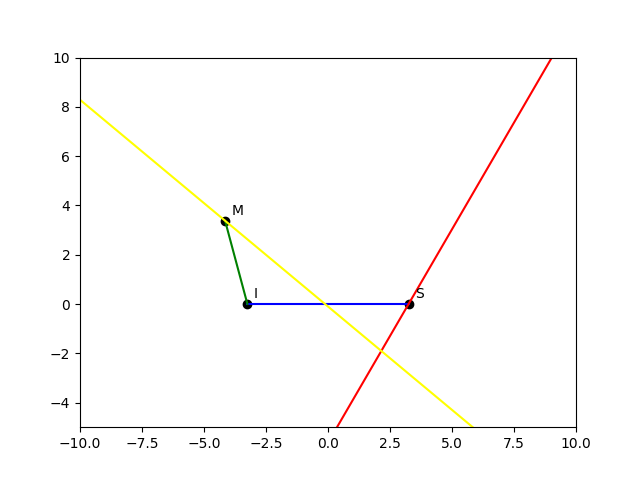
\includegraphics[scale = 0.52]{figure/Figure_1.png}
    \caption{Plot for Quadrilateral MIST}
    \label{fig:my_label}
\end{figure}

\end{document}
